%%%%%%%%%%%%%%%%%%%%%%%%%%%%%%%%%%%%%%%%%
% Beamer Presentation
% LaTeX Template
% Version 2.0 (March 8, 2022)
%
% This template originates from:
% https://www.LaTeXTemplates.com
%
% Author:
% Vel (vel@latextemplates.com)
%
% License:
% CC BY-NC-SA 4.0 (https://creativecommons.org/licenses/by-nc-sa/4.0/)
%
%%%%%%%%%%%%%%%%%%%%%%%%%%%%%%%%%%%%%%%%%

%----------------------------------------------------------------------------------------
%	PACKAGES AND OTHER DOCUMENT CONFIGURATIONS
%----------------------------------------------------------------------------------------

\documentclass[
	11pt, % Set the default font size, options include: 8pt, 9pt, 10pt, 11pt, 12pt, 14pt, 17pt, 20pt
	%t, % Uncomment to vertically align all slide content to the top of the slide, rather than the default centered
	%aspectratio=169, % Uncomment to set the aspect ratio to a 16:9 ratio which matches the aspect ratio of 1080p and 4K screens and projectors
]{beamer}

\graphicspath{{Images/}{./}} % Specifies where to look for included images (trailing slash required)

\usepackage{booktabs} % Allows the use of \toprule, \midrule and \bottomrule for better rules in tables

%----------------------------------------------------------------------------------------
%	SELECT LAYOUT THEME
%----------------------------------------------------------------------------------------

% Beamer comes with a number of default layout themes which change the colors and layouts of slides. Below is a list of all themes available, uncomment each in turn to see what they look like.

%\usetheme{default}
%\usetheme{AnnArbor}
%\usetheme{Antibes}
%\usetheme{Bergen}
%\usetheme{Berkeley}
%\usetheme{Berlin}
%\usetheme{Boadilla}
%\usetheme{CambridgeUS}
%\usetheme{Copenhagen}
%\usetheme{Darmstadt}
%\usetheme{Dresden}
%\usetheme{Frankfurt}
%\usetheme{Goettingen}
%\usetheme{Hannover}
%\usetheme{Ilmenau}
%\usetheme{JuanLesPins}
%\usetheme{Luebeck}
\usetheme{Madrid}
%\usetheme{Malmoe}
%\usetheme{Marburg}
%\usetheme{Montpellier}
%\usetheme{PaloAlto}
%\usetheme{Pittsburgh}
%\usetheme{Rochester}
%\usetheme{Singapore}
%\usetheme{Szeged}
%\usetheme{Warsaw}

%----------------------------------------------------------------------------------------
%	SELECT COLOR THEME
%----------------------------------------------------------------------------------------

% Beamer comes with a number of color themes that can be applied to any layout theme to change its colors. Uncomment each of these in turn to see how they change the colors of your selected layout theme.

%\usecolortheme{albatross}
%\usecolortheme{beaver}
%\usecolortheme{beetle}
%\usecolortheme{crane}
%\usecolortheme{dolphin}
%\usecolortheme{dove}
%\usecolortheme{fly}
%\usecolortheme{lily}
%\usecolortheme{monarca}
%\usecolortheme{seagull}
%\usecolortheme{seahorse}
%\usecolortheme{spruce}
%\usecolortheme{whale}
%\usecolortheme{wolverine}

%----------------------------------------------------------------------------------------
%	SELECT FONT THEME & FONTS
%----------------------------------------------------------------------------------------

% Beamer comes with several font themes to easily change the fonts used in various parts of the presentation. Review the comments beside each one to decide if you would like to use it. Note that additional options can be specified for several of these font themes, consult the beamer documentation for more information.

\usefonttheme{default} % Typeset using the default sans serif font
%\usefonttheme{serif} % Typeset using the default serif font (make sure a sans font isn't being set as the default font if you use this option!)
%\usefonttheme{structurebold} % Typeset important structure text (titles, headlines, footlines, sidebar, etc) in bold
%\usefonttheme{structureitalicserif} % Typeset important structure text (titles, headlines, footlines, sidebar, etc) in italic serif
%\usefonttheme{structuresmallcapsserif} % Typeset important structure text (titles, headlines, footlines, sidebar, etc) in small caps serif

%------------------------------------------------

%\usepackage{mathptmx} % Use the Times font for serif text
\usepackage{palatino} % Use the Palatino font for serif text

%\usepackage{helvet} % Use the Helvetica font for sans serif text
\usepackage[default]{opensans} % Use the Open Sans font for sans serif text
%\usepackage[default]{FiraSans} % Use the Fira Sans font for sans serif text
%\usepackage[default]{lato} % Use the Lato font for sans serif text

%----------------------------------------------------------------------------------------
%	SELECT INNER THEME
%----------------------------------------------------------------------------------------

% Inner themes change the styling of internal slide elements, for example: bullet points, blocks, bibliography entries, title pages, theorems, etc. Uncomment each theme in turn to see what changes it makes to your presentation.

%\useinnertheme{default}
\useinnertheme{circles}
%\useinnertheme{rectangles}
%\useinnertheme{rounded}
%\useinnertheme{inmargin}

%----------------------------------------------------------------------------------------
%	SELECT OUTER THEME
%----------------------------------------------------------------------------------------

% Outer themes change the overall layout of slides, such as: header and footer lines, sidebars and slide titles. Uncomment each theme in turn to see what changes it makes to your presentation.

%\useoutertheme{default}
%\useoutertheme{infolines}
%\useoutertheme{miniframes}
%\useoutertheme{smoothbars}
%\useoutertheme{sidebar}
%\useoutertheme{split}
%\useoutertheme{shadow}
%\useoutertheme{tree}
%\useoutertheme{smoothtree}

%\setbeamertemplate{footline} % Uncomment this line to remove the footer line in all slides
%\setbeamertemplate{footline}[page number] % Uncomment this line to replace the footer line in all slides with a simple slide count

%\setbeamertemplate{navigation symbols}{} % Uncomment this line to remove the navigation symbols from the bottom of all slides

%----------------------------------------------------------------------------------------
%	PRESENTATION INFORMATION
%----------------------------------------------------------------------------------------

\title[What is Agro-Informatics?]{What is Agro-Informatics?} % The short title in the optional parameter appears at the bottom of every slide, the full title in the main parameter is only on the title page

\subtitle{AEC3012} % Presentation subtitle, remove this command if a subtitle isn't required

\author[Hoyeon Jeong]{Hoyeon Jeong} % Presenter name(s), the optional parameter can contain a shortened version to appear on the bottom of every slide, while the main parameter will appear on the title slide

\institute[CNU]{Chonnam National University \\ \smallskip \textit{hjeong@jnu.ac.kr}} % Your institution, the optional parameter can be used for the institution shorthand and will appear on the bottom of every slide after author names, while the required parameter is used on the title slide and can include your email address or additional information on separate lines

\date[\today]{Dept. Agricultural Economics \\ \today} % Presentation date or conference/meeting name, the optional parameter can contain a shortened version to appear on the bottom of every slide, while the required parameter value is output to the title slide

%----------------------------------------------------------------------------------------

\begin{document}

%----------------------------------------------------------------------------------------
%	TITLE SLIDE
%----------------------------------------------------------------------------------------

\begin{frame}
	\titlepage % Output the title slide, automatically created using the text entered in the PRESENTATION INFORMATION block above
\end{frame}

%----------------------------------------------------------------------------------------
%	TABLE OF CONTENTS SLIDE
%----------------------------------------------------------------------------------------

% The table of contents outputs the sections and subsections that appear in your presentation, specified with the standard \section and \subsection commands. You may either display all sections and subsections on one slide with \tableofcontents, or display each section at a time on subsequent slides with \tableofcontents[pausesections]. The latter is useful if you want to step through each section and mention what you will discuss.

% Slide 1
\begin{frame}
	\frametitle{Agro-Informatics}
	
	\begin{block}{Food and Agriculture Organization (FAO)}
		Agro-informatics connects information technology with the farm management, analysis and application of agricultural data to design more accurate and targeted agricultural interventions.
	\end{block}
	
	\begin{exampleblock}{Examples of The Use of New Technology in Agriculture}
		 Satellite Imagery \\ 
		 Remote Sensing \\ 
		 Geographic Information Systems (GIS) \\ 
	\end{exampleblock}
	
	\begin{block}{Information and Technology in Agriculture}
		Information and Technology enable the transformation of data into actionable information.
	\end{block}
\end{frame}

% Slide 2
\begin{frame}
	\frametitle{Benefits of Agro-Informatics}
	\begin{itemize}
		\item Enhanced Decision Making: With real-time data on soil health, weather patterns, and crop growth, farmers can make informed decisions that maximize their yield.
		\item Resource Optimization: Agriculture informatics helps optimize the use of resources such as water, fertilizers, and pesticides, reducing waste and environmental impact.
		\item Precision Agriculture: Through GPS and remote sensing technologies, farmers can precisely target their interventions, minimizing costs and environmental harm.
	\end{itemize}
\end{frame}

% Slide 3
\begin{frame}
	\frametitle{Benefits of Agro-Informatics}
	\begin{itemize}
		\item Early Disease Detection: Monitoring tools and data analysis enable the early detection of disease outbreaks, preventing their spread and minimizing losses.
		\item Supply Chain Efficiency: Informatics streamlines the supply chain, reducing post-harvest losses and ensuring fresher produce reaches consumers.
	\end{itemize}
\end{frame}

% Slide 4
\begin{frame}
	\frametitle{Example of Agro-Informatics}
	\begin{figure}
		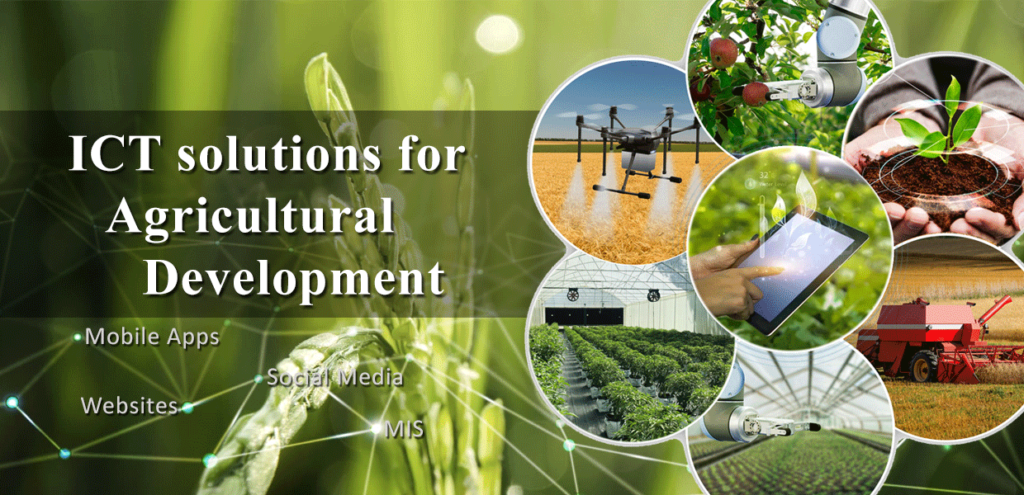
\includegraphics[width=0.8\linewidth]{images/figure1.png}
		\label{fig:https://doa.gov.lk/ict-solutions/}
	\end{figure}
\end{frame}

% Slide 5
\begin{frame}
	\frametitle{Example of Agro-Informatics}
	\begin{figure}
		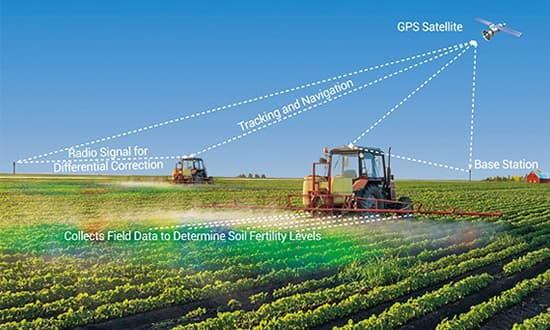
\includegraphics[width=0.8\linewidth]{images/figure2.png}
		\label{fig:https://www.vervetronics.com/solutions/iot-smart-agriculture/precision-agriculture/}
	\end{figure}
\end{frame}

% Slide 6
\begin{frame}
	\frametitle{Example of Agro-Informatics}
	\begin{figure}
		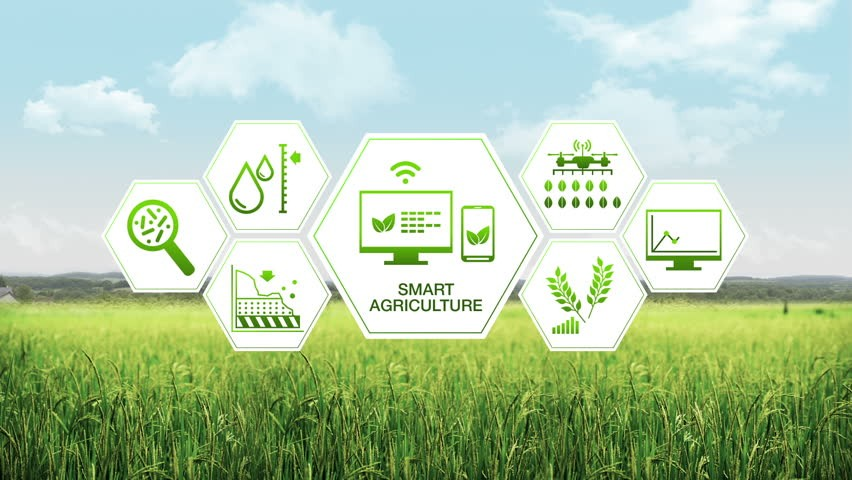
\includegraphics[width=0.8\linewidth]{images/figure3.jpg}
		\label{fig:https://www.linkedin.com/pulse/smart-farming-data-science-sanket-dayama}
	\end{figure}
\end{frame}

% Slide 7
\begin{frame}
	\frametitle{In this class,}
		\begin{itemize}
			\item We will combine agricultural economics and computer science.
			\item We will learn about how to collect, store, and analyze a variety of data used in agriculutural econmics.
		\end{itemize}
\end{frame}

% Slide 8
\begin{frame}
	\frametitle{Data Collect}
		\begin{itemize}
			\item A variety of sources of data and information related to agriculutral economics
			\item Statistics Korea, Bank of Korea, Government Agencies, AGRIX, etc
			\item International Agricultural Data (World Bank, FAO, etc)
		\end{itemize}
\end{frame}

% Slide 9
\begin{frame}
	\frametitle{KOSIS}
	\begin{figure}
		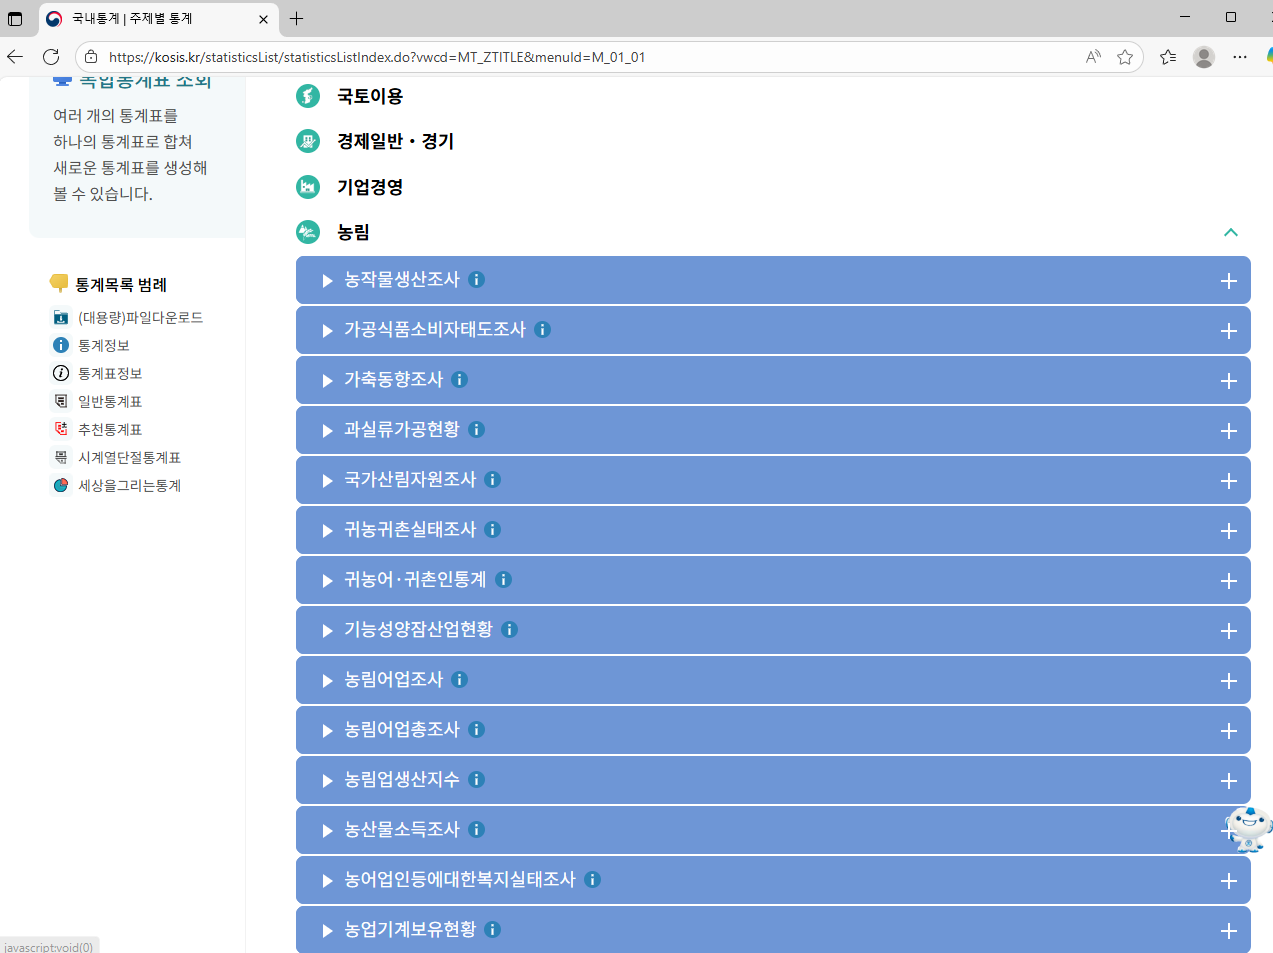
\includegraphics[width=0.8\linewidth]{images/figure4.png}
		\label{fig}
	\end{figure}
\end{frame}


% Slide 10
\begin{frame}
	\frametitle{KOSIS}
	\begin{figure}
		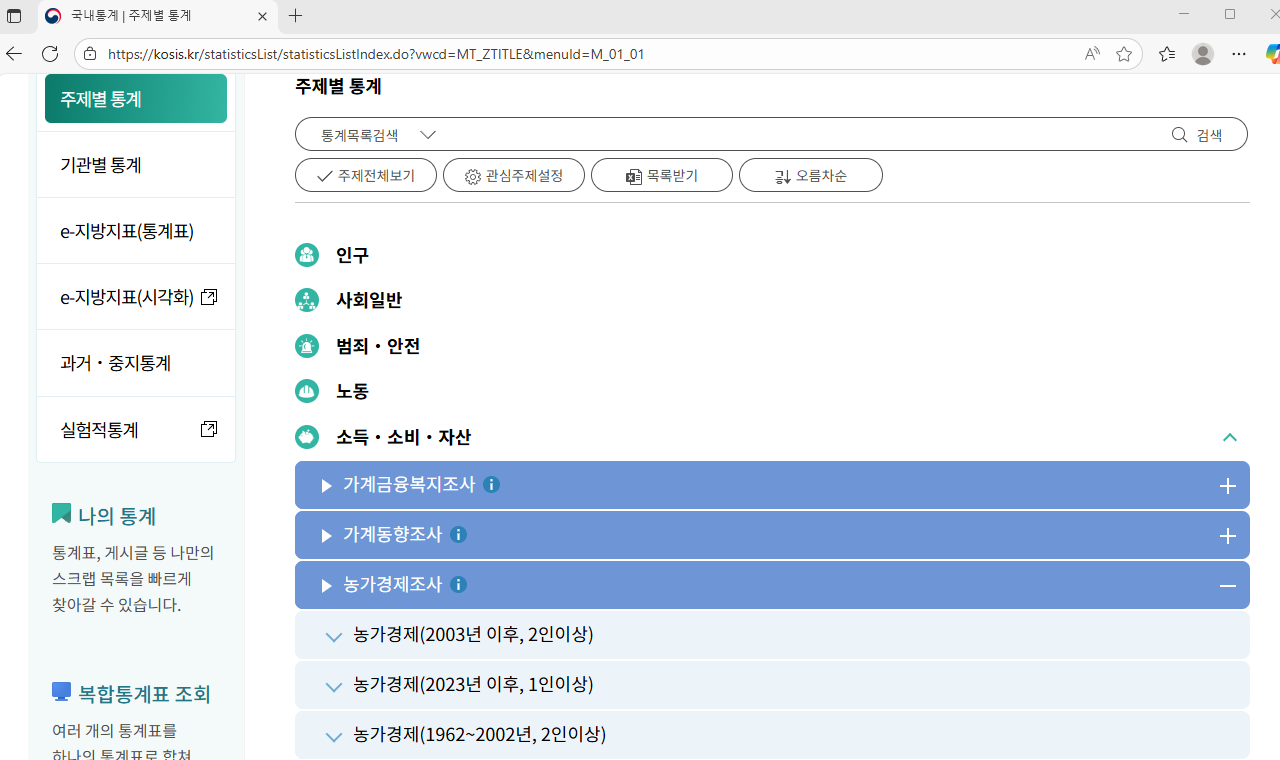
\includegraphics[width=0.8\linewidth]{images/figure5.png}
		\label{fig}
	\end{figure}
\end{frame}


% Slide 11
\begin{frame}
	\frametitle{AGRIX}
	\begin{figure}
		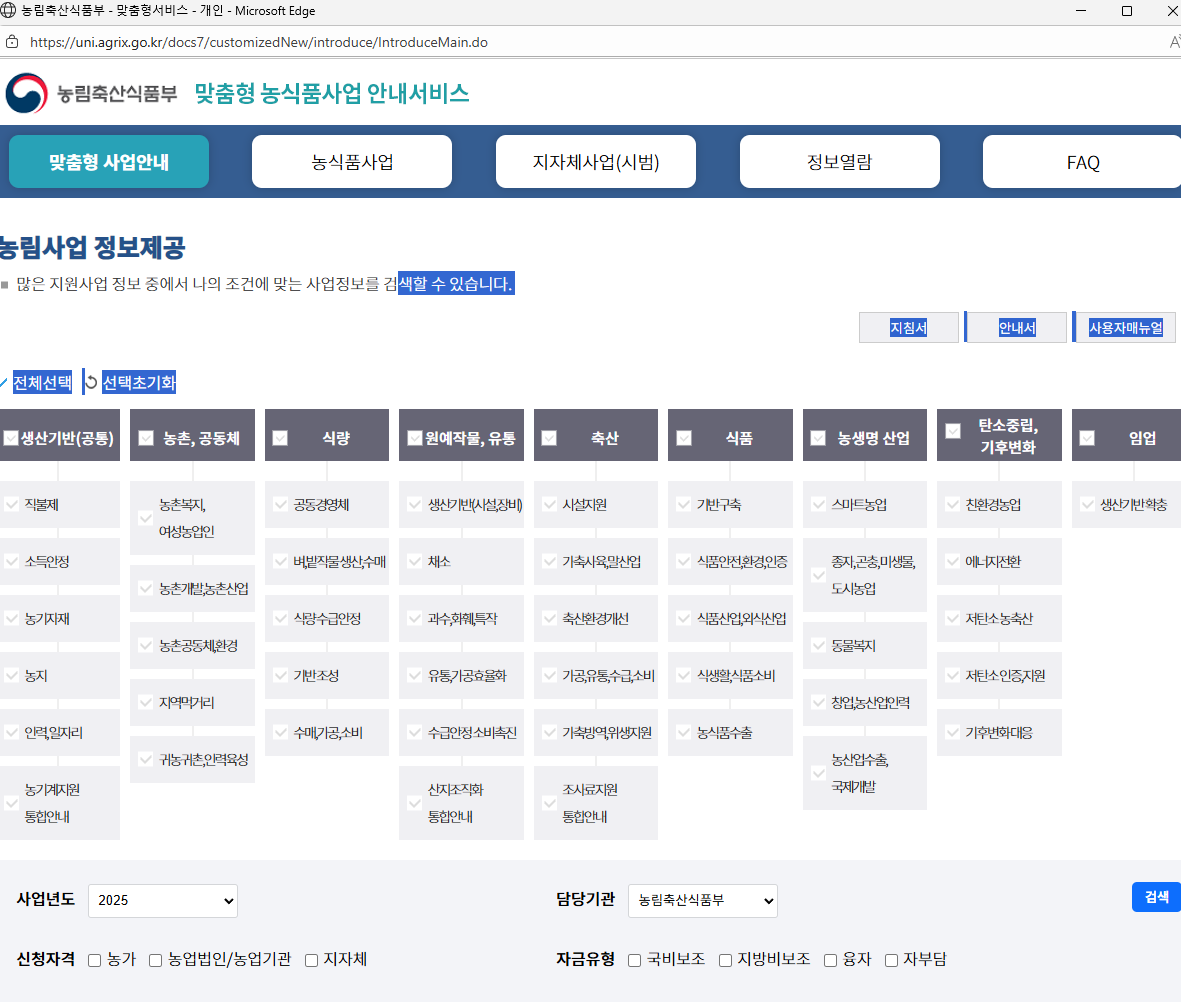
\includegraphics[width=0.8\linewidth]{images/figure6.png}
		\label{fig}
	\end{figure}
\end{frame}

% Slide 12
\begin{frame}
	\frametitle{World Bank Open Data}
	\begin{figure}
		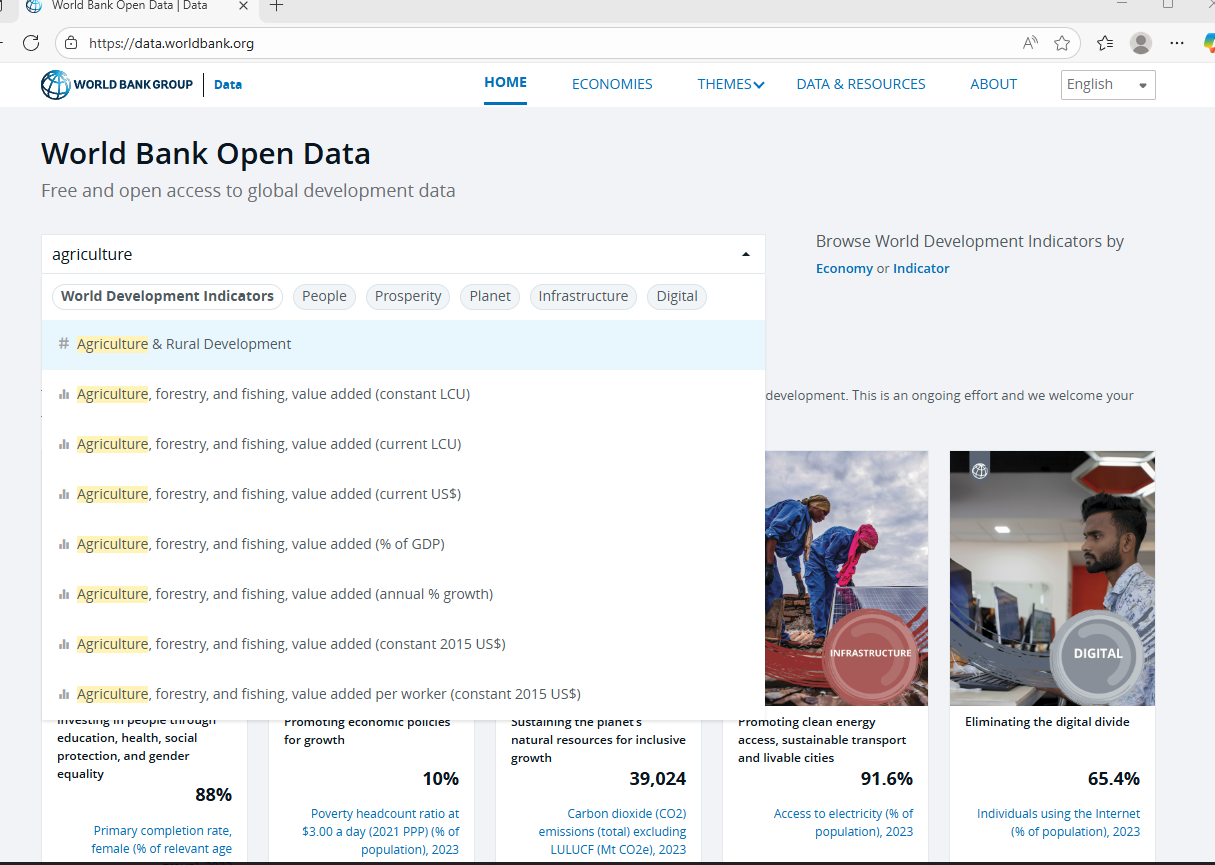
\includegraphics[width=0.8\linewidth]{images/figure7.png}
		\label{fig}
	\end{figure}
\end{frame}

% Slide 13
\begin{frame}
	\frametitle{FAOSTAT}
	\begin{figure}
		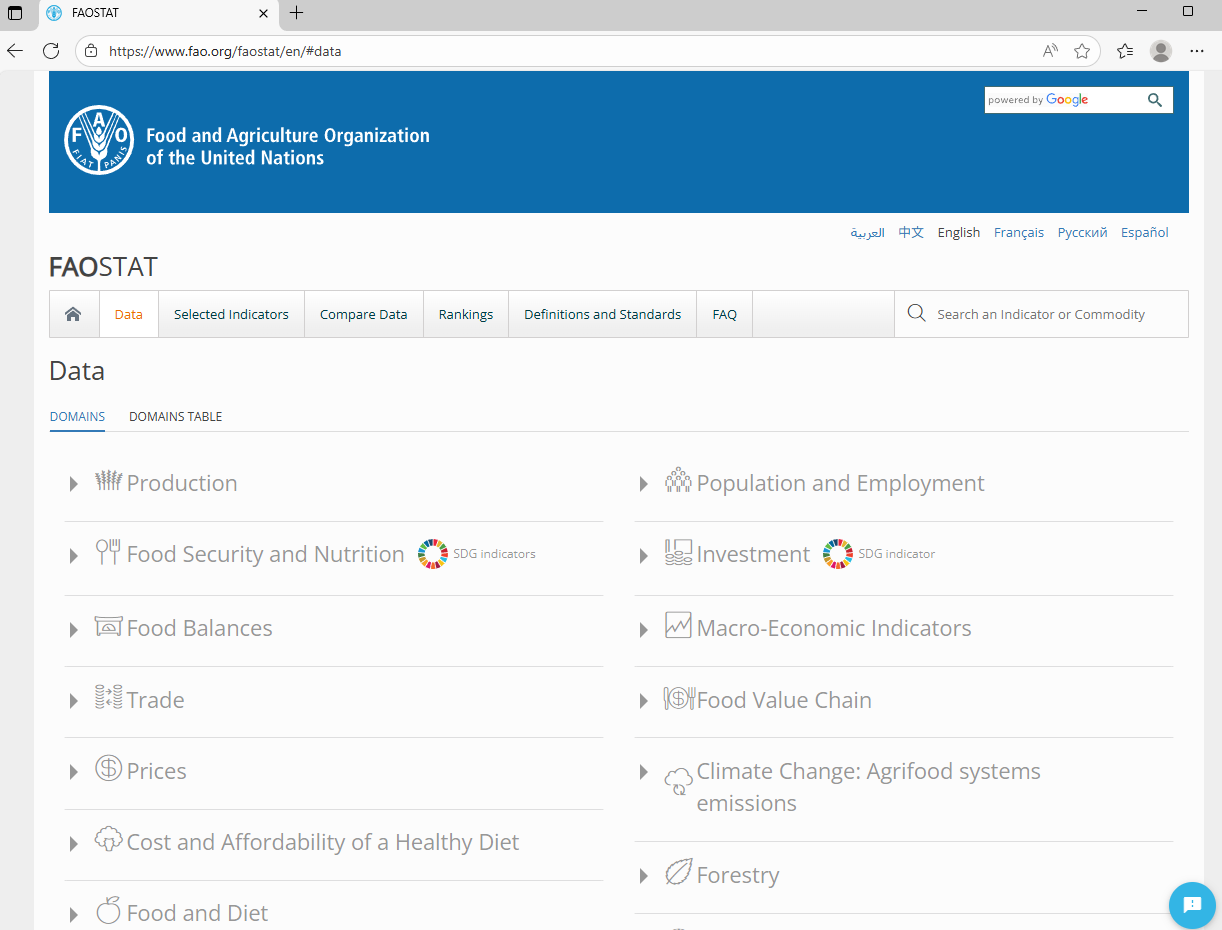
\includegraphics[width=0.8\linewidth]{images/figure8.png}
		\label{fig}
	\end{figure}
\end{frame}

% Slide 14
\begin{frame}
	\frametitle{Data Store}
		\begin{itemize}
			\item Database Management System (DBMS, e.g., MS ACESS)
			\item Enterprise Resource Planning (ERP)
			\item Structured Query Language (SQL)
		\end{itemize}
\end{frame}

% Slide 14
\begin{frame}
	\frametitle{DBMS}
	\begin{figure}
		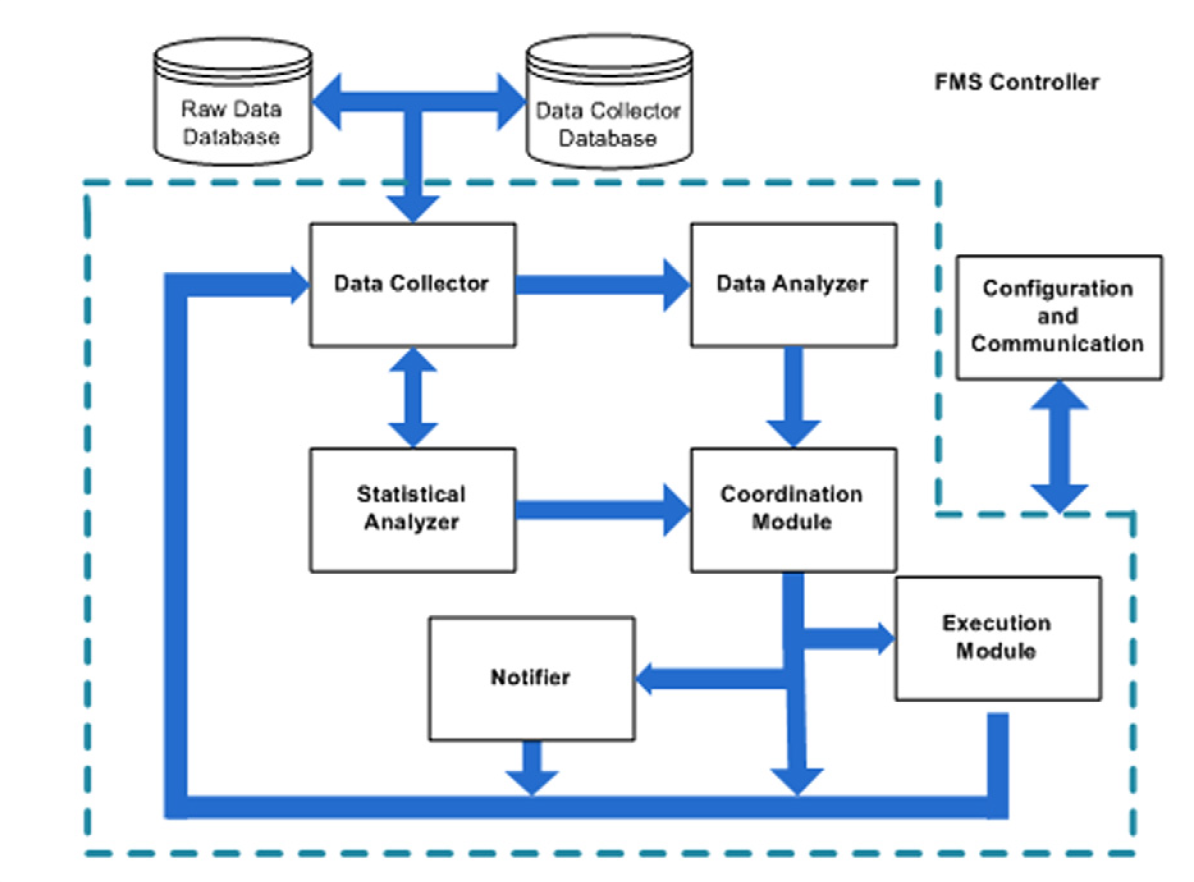
\includegraphics[width=0.8\linewidth]{images/figure9.png}
		\label{fig: Kaloxylos et al. 2012}
	\end{figure}
\end{frame}

% Slide 15
\begin{frame}
	\frametitle{DBMS}
	\begin{figure}
		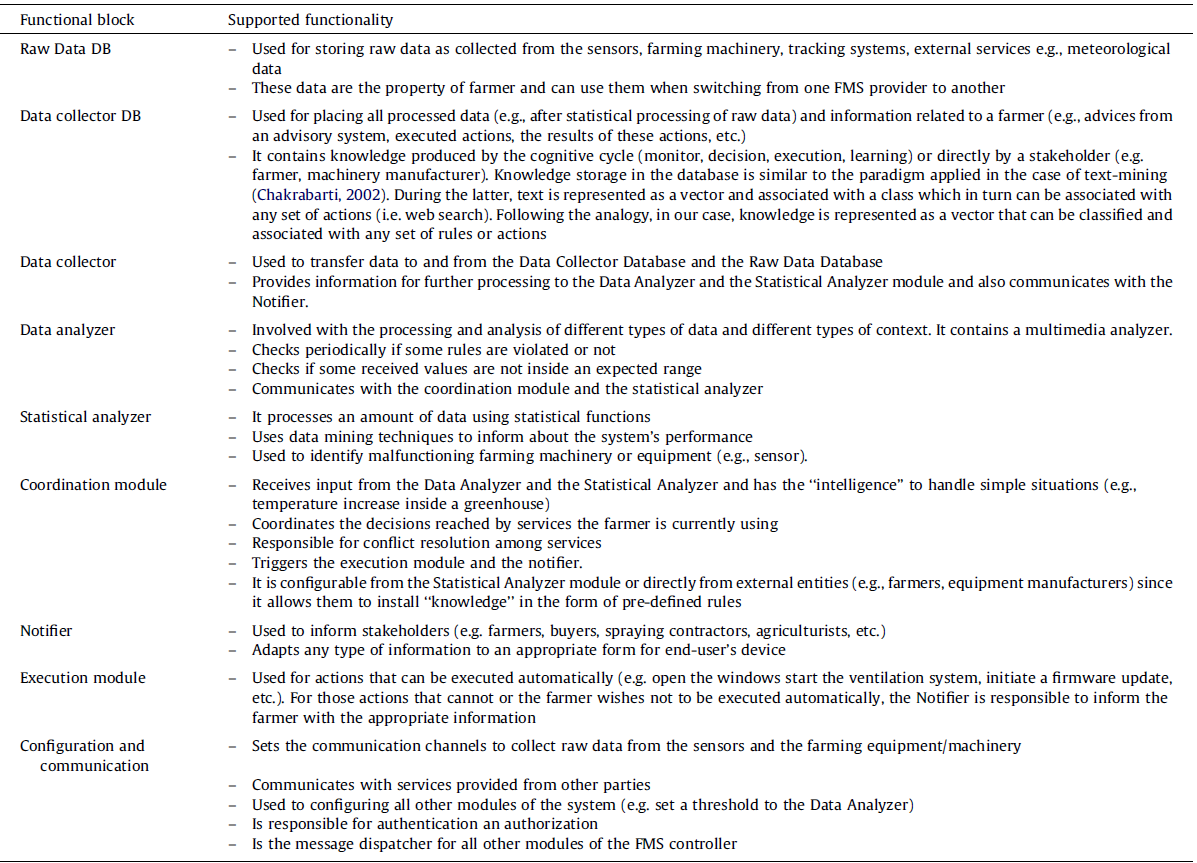
\includegraphics[width=0.8\linewidth]{images/figure10.png}
		\label{fig: Kaloxylos et al. 2012}
	\end{figure}
\end{frame}

% Slide 15
\begin{frame}
	\frametitle{ERP}
	\begin{figure}
		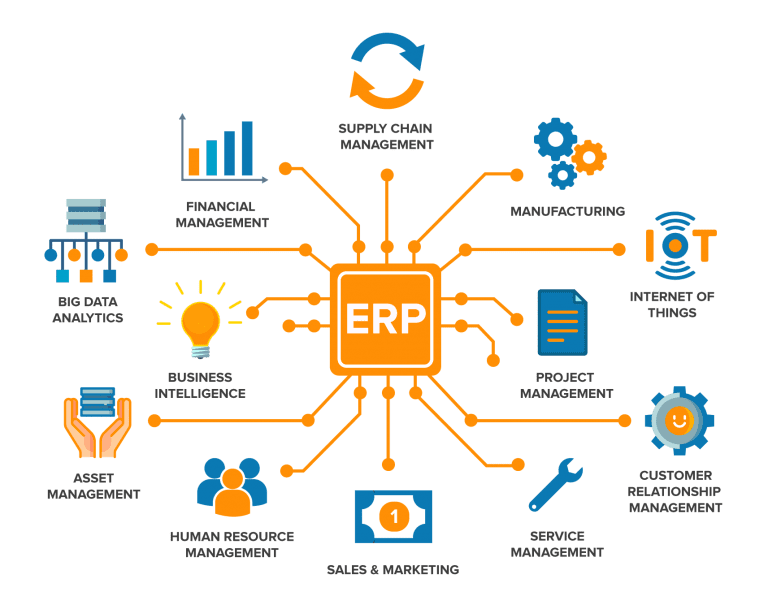
\includegraphics[width=0.8\linewidth]{images/figure11.png}
		\label{fig:https://www.finereport.com}
	\end{figure}
\end{frame}

% Slide 16
\begin{frame}
	\frametitle{SQL}
	\begin{figure}
		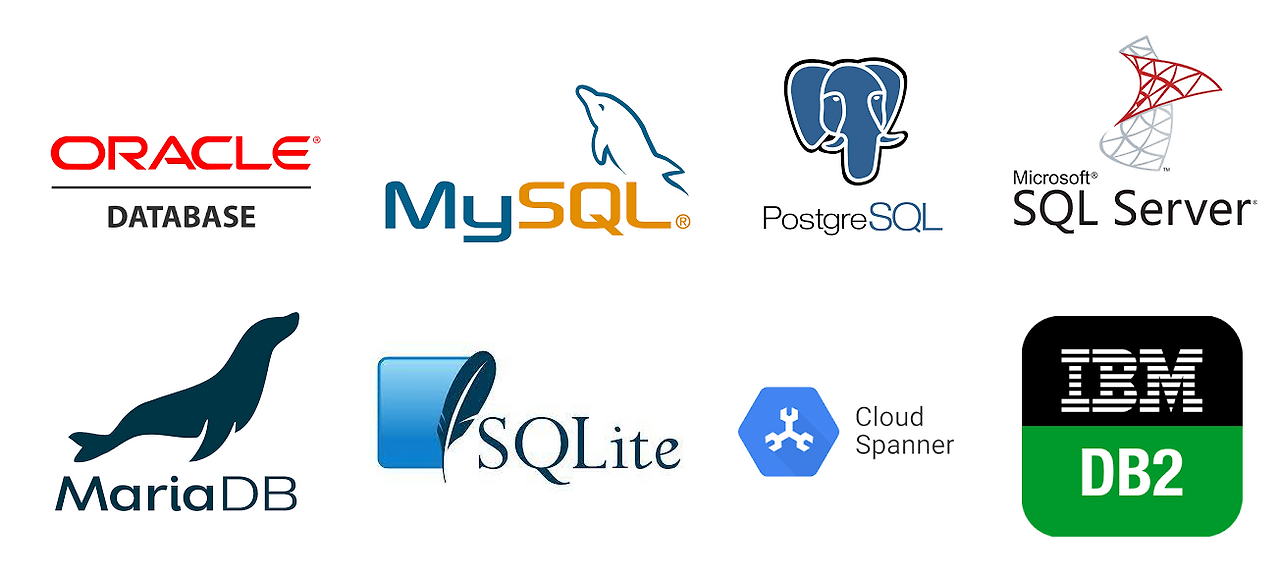
\includegraphics[width=0.8\linewidth]{images/figure12.png}
		\label{fig:https://miny-genie.tistory.com/262}
	\end{figure}
\end{frame}

% Slide 17
\begin{frame}
	\frametitle{Data Analysis}
		\begin{itemize}
			\item Data: Raw, unorganized (unprocessed) facts that need context to become useful
			\item Information: Processed, organized, interpreted and analyzed data used for specific purposes (e.g., descision-making) by adding meaning and value
			\item Data is used for information, which is also can be used for other information.
		\end{itemize}
\end{frame}

% Slide 18
\begin{frame}
	\frametitle{Data Becomes Information}
	\begin{figure}
		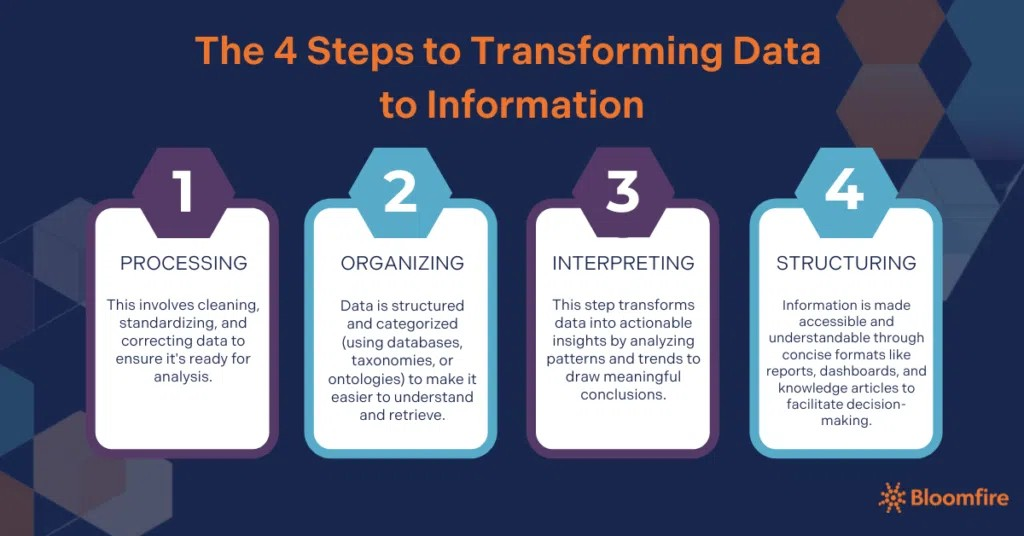
\includegraphics[width=0.8\linewidth]{images/figure13.png}
		\label{fig:}
	\end{figure}
\end{frame}

%----------------------------------------------------------------------------------------
\end{document} 